\documentclass[11p]{article}
% Packages
\usepackage{amsmath}
\usepackage{graphicx}
\usepackage{fancyheadings}
\usepackage[swedish]{babel}
\usepackage[
    backend=biber,
    style=authoryear-ibid,
    sorting=ynt
]{biblatex}
\usepackage[utf8]{inputenc}
\usepackage[T1]{fontenc}
%Källor
\addbibresource{references.bib}
\graphicspath{ {./images/} }

% Lite variabler
\def\email{levi.hogdal@ga.ntig.se}
\def\foottitle{PMmall}
\def\name{Levi Högdal}

\title{PMmall \\ \small Gymnasiearbete}
\author{\name}
\date{\today}

\begin{document}

% fixar sidfot
\lfoot{\footnotesize{\name \\ \email}}
\rfoot{\footnotesize{\today}}
\lhead{\sc\footnotesize\foottitle}
\rhead{\nouppercase{\sc\footnotesize\leftmark}}
\pagestyle{fancy}
\renewcommand{\headrulewidth}{0.2pt}
\renewcommand{\footrulewidth}{0.2pt}

% i Sverige har vi normalt inget indrag vid nytt stycke
\setlength{\parindent}{0pt}
% men däremot lite mellanrum
\setlength{\parskip}{10pt}

\maketitle

\newpage

\section{Bakgrund}

\subsection{Användarbarhet}

\subsection{Tillgänglighet}
Tillgänglighet i det här sammanhanget betyder inte hur åtkomligt något ska vara utom att saker ska kunna användas av alla personer även de med funktionsnedsättning.
Tillgänglighet handlar om saker som hur bra kontrast det är mellan bakgrund och text så att det ska vara enkelt att läsa texten och har bilder en bildtext, inte kan jag komma åt hemsidan \parencite{webbriktlinjer}.
Webbsidor design och utformning ska vara anpassad så att alla människor ska kunna använda och förstå hemsidan så länge de kan läsa språket.
För att hemsidor ska se vettiga ut och användas av folk med funktionsnedsättningar så görs standarder som man kan följa när man skapar hemsidor och olika lagar.
Webbstandarden som den här undersökningen kommer hålla sig till är WCAG.

\subsection{WCAG 2.0}
WCAG är en webbstandard som är skapad av W3C.
Enligt \textcite{W3C} är W3C ett företag som grundades 1994 av Tim Berners-Lee för att säkerställa webbens utveckling och framtid.
För att åstadkomma det målet släpper W3C olika standarder och riktlinjer för webben.
WCAG 2.0 är en samling av olika rekommendationer som alla ska kunnas testas separat och inte riktas mot någon specific teknologi utan webben skännerält. \parencite{WCAG_2.0}



Riktlinjerna ska kunna testas på en hemsida oberoende hur hemsidan är uppbyggd.

\subsubsection{Varför WCAG 2.0}

\subsection{Lagar}
I sverige finns en lag som heter "Lagen om tillgänglighet till digital offentlig service (DOS-lagen)".\parencite{Dos-lagen}
Lagen ställer krav på offentliga aktörer så att de ska tillgänglighetsanpassa webbplatser och mobila application.

\subsubsection{Offentlig aktör}
Hur en offentlig aktör definieras finns förklarat i \textcite{Dos-lagen}.
Det kan enklare förklaras som offentlig information från staten som Statliga och kommunala myndigheter samt sammanslutningar till dem.
Saker som rör utbildning, skola, sjukvård ock omsorg måste också följa lagen.
Även om det ägs privat så kommer de behöva följa kraven från Dos-lagen.

Det kan enklare förklaras som statliga och kommunala myndigheter, beslutstagande församlingar i kommuner och regioner, skola och sjukvård.\parencite{Om_Dos-lage}


\subsection{Verktyg}

\subsection{Valda Hemsidor}


\section{Referenser}
Referenser i text kan skrivas på två sätt: Enligt \textcite{} kan man använde två typer av referenser, inbäddade i texten eller ``efter'' ett fakta \parencite{Fraenkel}. Ett till test för att se hur det ser ut \parencite{fermi}.

\section{Annat som kan vara bra att veta}
Det är lätt att skriva matematik i \LaTeX

\begin{equation}
    F = G \frac{M m}{r^2}
    \label{eq:grav}
\end{equation}

Ekvation (\ref{eq:grav}) känner ni igen...
\clearpage
\subsection{En underrubrik}
    \begin{figure}[!h]
        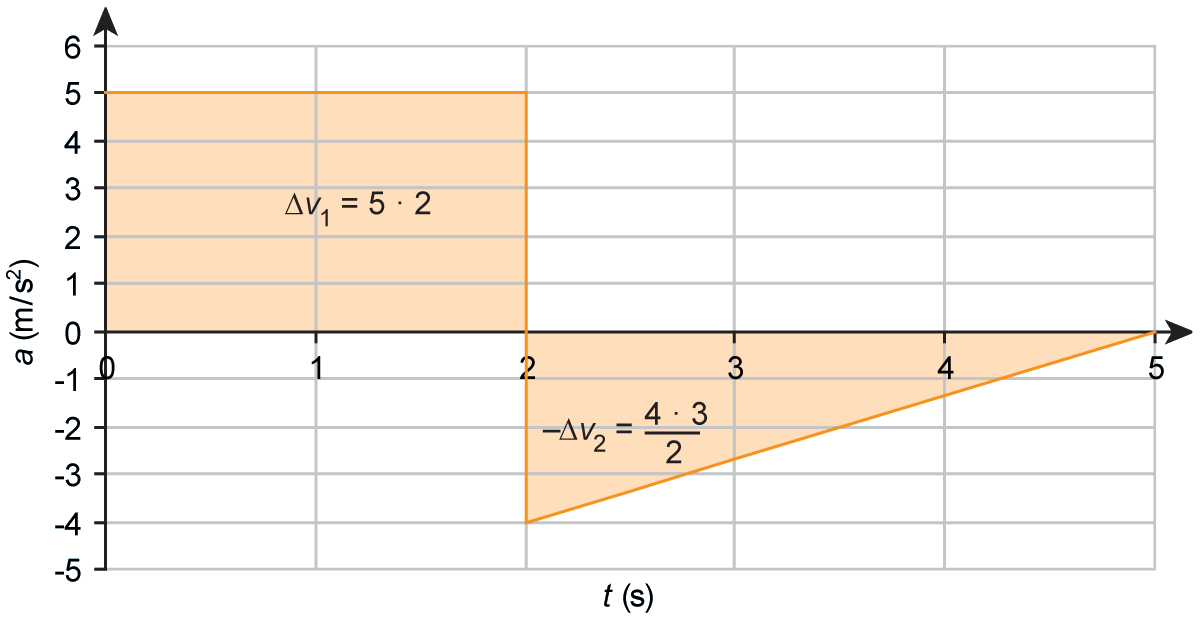
\includegraphics[width=0.8\textwidth]{accelerationTime.png}
        \caption{Acceleration-tid diagram. Källa: \textcite{Fraenkel}}
        \label{fig:acc}
    \end{figure}

Acceleration-tiddiagram (se figur \ref{fig:acc})

\printbibliography

\end{document}
